\documentclass{beamer}

\mode<presentation> {
}

\usepackage{graphicx} % Allows including images
\usepackage{booktabs} % Allows the use of \toprule, 
\usepackage{longtable} % Allows the use of \toprule, 



\title[]{Bayesian Clinical Trials} 
\subtitle{Dose Finding CRM} 
\date{} 


\begin{document}

\begin{frame}
\titlepage % Print the title page as the first slide
\end{frame}


\begin{frame}{Phase I study}

Goals:

\begin{enumerate}
\def\labelenumi{\arabic{enumi}.}
\itemsep1pt\parskip0pt\parsep0pt
\item
  Determine a safe dose for further clinical studied
\item
  Study pharmacokinetics of the drug
\end{enumerate}

\end{frame}

\begin{frame}{Toxicity Dose-Response Curve}

We can ordinarily assume that the probability of a dose-limiting adverse
event increases {monotonically} with dose

In that circumstances, the {Maximum Tolerated Dose (MTD)} is the dose
associated with the specified probability of a {dose-limiting toxicity
(DLT)}

\end{frame}

\begin{frame}{Diagram of Dose Response Relationship}

\begin{center}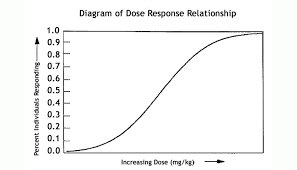
\includegraphics[scale=0.8]{images/Dose-Response.png} \end{center}

\href{https://www.osha.gov/pls/oshaweb/owadisp.show_document?p_id=770\&p_table=preambles}{Health
Effects Discussion and Determination of Final PEL, OSHA}

\end{frame}

\begin{frame}{Diagram of Dose Response Relationship}

\begin{center}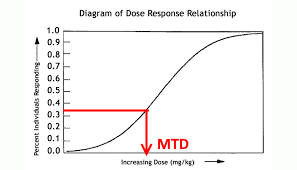
\includegraphics[scale=1.5]{images/Dose-Response_2.png} \end{center}


\href{https://www.osha.gov/pls/oshaweb/owadisp.show_document?p_id=770\&p_table=preambles}{Health
Effects Discussion and Determination of Final PEL, OSHA}

\end{frame}

\begin{frame}{Rules based models}

\begin{itemize}
\itemsep1pt\parskip0pt\parsep0pt
\item
  Make no assumptions about the form of the dose-toxicity curve
\item
  Often called ``up-and-down'' designs because they allow dose
  escalation and de-escalation
\item
  The dose is increased or decreased depending on the occurrence of
  dose-limiting toxicities (DLT)
\item
  More than 90\% or Phase I trials in cancer are rule-based (\emph{J
  Natl Cancer Inst 2009; 101:708-720})
\end{itemize}

\end{frame}

\begin{frame}{Conventional 3+3 Design}

\begin{center}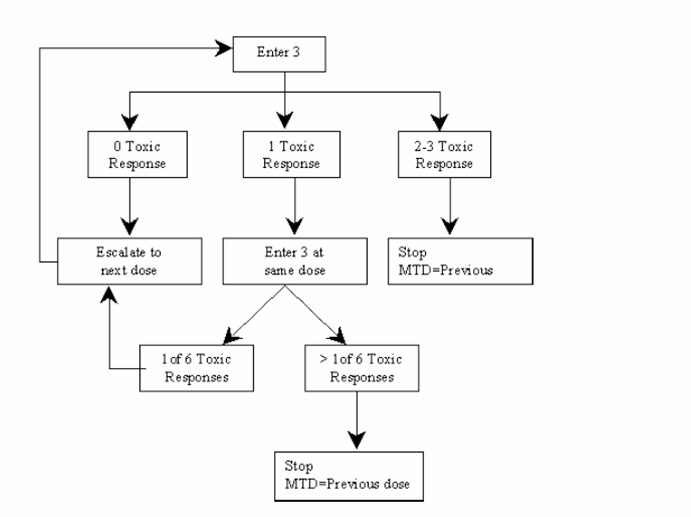
\includegraphics[scale=0.4]{images/Conventional3+3.png} \end{center}

\end{frame}

\begin{frame}{Model Based Design}

\begin{itemize}
\itemsep1pt\parskip0pt\parsep0pt
\item
  Specify a mathematical model for dose-response curve
\item
  Choose the initial dose based on expert opinion
\item
  After each dose, re-estimate the model and choose the next dose as the
  dose estimated to have the specified probability of a DLT, eg. 0.33
\end{itemize}

\end{frame}

\begin{frame}{Model Based Design}

One popular model is the {logistic model}, which has only two
parameters, an intercept and a slope

\begin{center}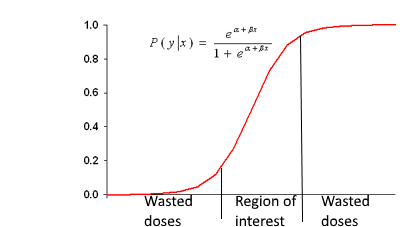
\includegraphics[scale=1.2]{images/logisticRegression.png} \end{center}


\end{frame}

\begin{frame}{Comparing Rule and Model-Based Design}

\begin{longtable}[c]{@{}ll@{}}
\toprule
Rule Based Design & Model Based Designs\tabularnewline
\midrule
\endhead
Easy to describe & Difficult to describe\tabularnewline
Easy to implement & Require statistical support\tabularnewline
Possibly inefficient & May be more efficient\tabularnewline
\bottomrule
\end{longtable}

\end{frame}

\begin{frame}{Outcome adaptive statistical models}

\begin{itemize}
\itemsep1pt\parskip0pt\parsep0pt
\item
  Continual Reassessment method
\item
  Bayesian Logistic Regression
\end{itemize}

They incorporate uncertainty regarding patient outcome by using Bayesian
probability models:

\begin{itemize}
\itemsep1pt\parskip0pt\parsep0pt
\item
  learning from accruing data
\item
  choosing doses for successive patient cohorts
\item
  describing various probabilities graphically
\end{itemize}

\end{frame}

\begin{frame}{Illustrative Trial: Renal Cell Carcinoma (RCC) Trial}

\begin{itemize}
\item
  Patients with renal cell carcinoma (RCC) that was progressive after
  previous treatment with interferon were eligible.
\item
  Treatment consisted of fixed doses of 5-Fluorouracil (5-FU) and
  interferon, plus one of six doses of gemcitabine (GEM):

  \begin{itemize}
  \itemsep1pt\parskip0pt\parsep0pt
  \item
    100, 200, 300, 400, 500 or 600mg/m2.
  \end{itemize}
\item
  Toxicity was defined as grade 3 or 4 diarrhea, mucositis, or
  hematologic toxicity.
\item
  A total of 36 patients were treated in cohorts of size 3, with the
  first cohort given 200mg/m2 of GEM.
\end{itemize}

\end{frame}

\begin{frame}{Dose Toxicity Probability Models}

The probability of toxicity \(P_{TOX}\) depends on the dose given to the
patient \[
P_{TOX}(100) < P_{TOX}(200) < \ldots < P_{TOX}(600)
\]

\textbf{underlying assumption:} a larger dose necessarily implies a
greater risk of toxicity, e.g \(P_{TOX}(dose)\) must increase with dose

\begin{columns}
\begin{column}{6cm}

\begin{center}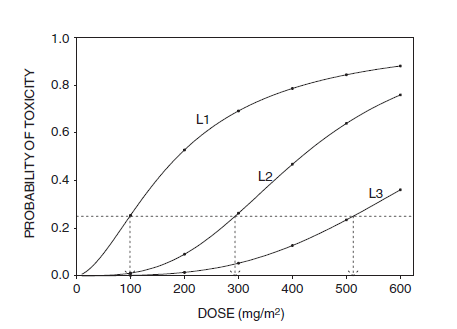
\includegraphics[scale=0.5]{images/BLR.png} \end{center}
\end{column}

\begin{column}{6cm}
Three possible dose-toxicity probability curves described by the
logistic regression model

\end{column}


\end{columns}

\end{frame}

\begin{frame}{Dose Toxicity Probability Models}

A model based method requires specifying a fixed \(P_{TOX}\) value as
\emph{target} for the dose-finding problem. In the RCC trial, the target
is 0.25:

\begin{itemize}
\itemsep1pt\parskip0pt\parsep0pt
\item
  it is clinically acceptable if on average 1 patient in 4 receiving the
  treatment at the MTD experiences toxicity

  \begin{itemize}
  \itemsep1pt\parskip0pt\parsep0pt
  \item
    targets in the range 0.10 to 0.40 are usually specified (the
    particular value varies depending on the definition of toxicity, the
    disease, the trial's entry criteria)
  \end{itemize}
\end{itemize}

\end{frame}

\begin{frame}{Bayesian Logistic Regression}

The Bayesian regression model has linear term \[
\eta(x,\theta) = \mu +\beta x, \qquad \mu\in R, \beta>0
\] which is linked to the probability toxicity \(\pi(d,\theta)\) by a
suitable link function \[
\pi(d,\theta) = g^{-1}\{\eta (x_j, \theta)\}, \qquad g(\pi) = \log\frac{\pi}{1-\pi}
\]

To determine the prior on \((\mu, \beta)\) elicited prior means
\(\pi(d_1,\theta)\) and \(\pi(d_2,\theta)\) at two distinct doses
\(d_1\) and \(d_2\) are used to determine priors on \((\mu, \beta)\).

\end{frame}

\begin{frame}{Bayesian Logistic Regression: simplified prior elicitation
approach}

A simpler approach can be adopted:

\begin{itemize}
\itemsep1pt\parskip0pt\parsep0pt
\item
  \(\mu\) and \(\beta\) are assumed independent normal
\item
  solves for the means of \(\mu\) and \(\beta\) based on elicited
  \(\pi(d_1,\theta)\) and \(\pi(d_2,\theta)\)
\item
  choose their variances to obtain a vague prior
\end{itemize}

\end{frame}

\begin{frame}{Bayesian Logistic Regression: simplified prior elicitation
approach}

\[
\pi(d_1,\theta) = g^{-1}\{\eta (x_j, \theta)\} = g^{-1}(\mu -0.18\beta) = 0.25 
\]

\[
\pi(d_2,\theta) = g^{-1}\{\eta (x_j, \theta)\} = g^{-1}(\mu + 0.22\beta) = 0.75 
\]

given doses \(d_1 < d_2 < \ldots < d_k\), \(x_j\) is the standardized
dose \(x_j = \log(d_j)-\frac{\log(d_1)+\ldots +\log(d_k)}{k}\). Thus
\(d_1=200, x_1 = -0.18\) and \(d_2 = 500, x_2 = 0.22\)

Solving (1) and (2): \[
E(\mu)=-0.1313, \qquad E(\beta)=2.3980
\] We chose \(\sigma_\mu = \sigma_\beta = 2\)

\end{frame}

\begin{frame}{Example}

\begin{center}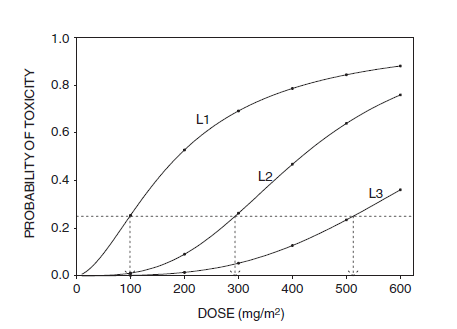
\includegraphics[scale=0.8]{images/BLR.png} \end{center}

\end{frame}

\begin{frame}{RCC Trial}

\begin{itemize}
\item
  Patients with renal cell carcinoma (RCC) that was progressive after
  previous treatment with interferon were eligible.
\item
  Treatment consisted of fixed doses of 5-Fluorouracil (5-FU) and
  interferon, plus one of six doses of gemcitabine (GEM):

  \begin{itemize}
  \itemsep1pt\parskip0pt\parsep0pt
  \item
    100, 200, 300, 400, 500 or 600mg/m2.
  \end{itemize}
\item
  Toxicity was defined as grade 3 or 4 diarrhea, mucositis, or
  hematologic toxicity.
\item
  A total of 36 patients were treated in cohorts of size 3, with the
  first cohort given 200mg/m2 of GEM.
\end{itemize}

\end{frame}

\begin{frame}{Continual Reassessment Method (CRM)}

\begin{itemize}
\itemsep1pt\parskip0pt\parsep0pt
\item
  Model-based Bayesian method introduced by J. O'Quigley
  (\emph{Biometrics} 1990)
\item
  Parametric model for dose-response relationship and fixed target for
  \(P_{TOX}\)
\item
  It requires a skeleton of fixed probabilities corresponding to the
  dose levels
\item
  It requires prior information
\item
  The study begins by dosing the first patient at the \emph{best} dose
\item
  The analysis is updated given the data obtained
\item
  For the next patient pick the ``best'' dose and continue
\end{itemize}

\end{frame}

\begin{frame}{CRM: single parameter working model}

\[
P(d, \alpha) = \rm{probability\  of \ a \ toxicity\ at\ dose\ d}
\]

The following working models were suggested in (Biometrics 1990)

\begin{itemize}
\itemsep1pt\parskip0pt\parsep0pt
\item
  1- parameter logistic:
  \(P(d,\theta) = \frac{\exp(-3+\theta d)}{1+ \exp(-3+\theta d)}\)
\item
  power: \(P(d,\theta) = d^{\exp(\theta)}\)
\item
  hyperbolic tangent:
  \(P(d,\theta) = \left(\frac{\exp(d)}{\exp(d)+\exp(-d)}\right)^\theta\)
\end{itemize}

\end{frame}

\begin{frame}{CRM: Prior information}

\(\alpha\) is the parameter that is going to be updated during the trial

\begin{itemize}
\itemsep1pt\parskip0pt\parsep0pt
\item
  exponential prior \(\pi(\theta) =\exp(-\theta)\) with mean 1
\item
  normal prior \(\pi(\theta)=Normal(0,var(\theta))\) with
  \(1\leq var(\theta) \leq 10\)
\end{itemize}

Given the data for doses \(x_i\) and outcomes \(y_i\), the likelihood is

\[
f(x\vert\theta) = \prod_i P(x_i,\theta)^{y_i}(1-P(x_i,\theta))^{1-y_i}
\]

and the posterior is

\[
\pi(\theta\vert x) = \frac{f(x\vert\theta)\pi(\theta)}{\int_0^\infty f(x\vert\theta)\pi(\theta)d\theta}
\] computed by numerical integration or MCMC methods

\end{frame}

\begin{frame}{Example: RCC trial}

\begin{itemize}
\itemsep1pt\parskip0pt\parsep0pt
\item
  The prior probabilities for each toxicity (\emph{skeleton}) for 6 dose
  levels need to be specified
\end{itemize}

\begin{longtable}{lcccccc}
\toprule
doses & \(100\) & \(200\) & \(300\) & \(400\) &
\(500\) & \(600\)\tabularnewline
probabilities & 0.15 & 0.25 & 0.40 & 0.60 & 0.75 & 0.85\tabularnewline
\bottomrule
\end{longtable}

 The skeleton is fixed throughout the trial and dictates the shape of
the curve

\begin{itemize}
\itemsep1pt\parskip0pt\parsep0pt
\item
  Target (TTL) is specified at 0.25
\item
  Default working model is exponential
\item
  Default prior is Normal(0, 1.8)
\end{itemize}

\end{frame}

\begin{frame}{CRM}
\begin{center}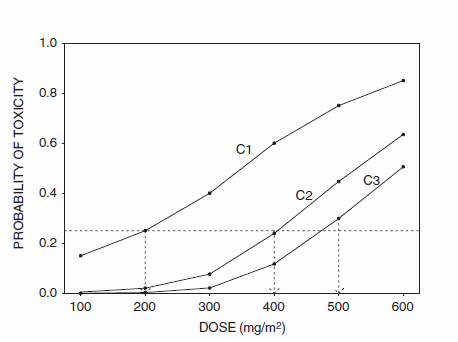
\includegraphics[scale=0.8]{images/CRM.png} \end{center}

\end{frame}

\begin{frame}{CRM}

Under either model:

\begin{itemize}
\itemsep1pt\parskip0pt\parsep0pt
\item
  denoting \(Y_i=1\) if the ith patient suffers toxicity
\item
  denoting \(Y_i=0\) if not,
\item
  denoting \(d(i)\) that patient's dose
\end{itemize}

the likelihood for n patients is

\[
\prod_{i=1}^n \pi(d_i,\theta)^{Y_i}\times (1-\pi(d_i,\theta ))^{(1-Y_i)}
\]

The posterior of \(\theta\) and each posterior mean
\(E(\pi(d_j, \theta)|data)\) may be computed using either numerical
integration or Markov chain Monte Carlo methods.

\end{frame}

\begin{frame}{CRM stopping rules}

The additional rule that stops the trial if the lowest dose is
excessively toxic is given formally by \[
Prob\{\pi(d_1, \theta) > \pi^*|data\} > p_U
\] where \(p^*\) is the fixed target and \(p_U\) is a fixed upper
probability cut-off, usually in the range 0.95 to 0.99.

\end{frame}

\begin{frame}{References}

\begin{itemize}
\item Thall, P. F. and Lee, S.-J. (2003), Practical model-based dose-finding in phase I clinical trials: Methods based on toxicity. International Journal of Gynecological Cancer, 13: 251–261

\item
  O'Quigley J, Pepe M, Fisher L. Continual reassessment method: a
  practical design for phase I clinical trials in cancer. Biometrics
  1990; 46: 33-48.
  
  \item
  Le Tourneau C, Lee JJ, Siu LL. Dose Escalation Methods in Phase I Cancer Clinical Trials. JNCI Journal of the National Cancer Institute. 2009;101(10):708-720. 
  
  \end{itemize}
\end{frame}

\end{document}